\documentclass{article}
\usepackage[utf8]{inputenc} %кодировка
\usepackage[T2A]{fontenc}
\usepackage[english,russian]{babel} %русификатор 
\usepackage{mathtools} %библиотека матеши
\usepackage[left=1cm,right=1cm,top=2cm,bottom=2cm,bindingoffset=0cm]{geometry} %изменение отступов на листе
\usepackage{amsmath}
\usepackage{graphicx} %библиотека для графики и картинок
\graphicspath{}
\DeclareGraphicsExtensions{.pdf,.png,.jpg}
\usepackage{subcaption}
\usepackage{pgfplots}
\usepackage{derivative}
\usepackage{amsfonts}
\usepackage{esint}

\usepackage{graphicx}
\graphicspath{ {images/} }
\usepackage{float} % чтобы можно было указывать H и размещать изображения где мне надо

% подключаем hyperref (для ссылок внутри  pdf)
\usepackage[unicode, pdftex]{hyperref}
\graphicspath{ {./} }

\usepackage{float}

\graphicspath{{./}}
\newcommand{\Mod}[1]{\ \mathrm{mod}\ #1}


\begin{document}
% НАЧАЛО ТИТУЛЬНОГО ЛИСТА
\begin{center}
    \Large
    Федеральное государственное автономное \\
    образовательное учреждение высшего образования \\ 
    «Научно-образовательная корпорация ИТМО»\\
    \vspace{0.5cm}
    \large
    Факультет программной инженерии и компьютерной техники \\
    Направление подготовки 09.03.04 Программная инженерия \\
    \vspace{1cm}
    \Large
    \textbf{Отчёт по расчетно-графической работе №5} \\
    По дисциплине «Математический анализ» (третий семестр)\\
    \large
    \vspace{8cm}

    \begin{minipage}{.33\textwidth}
    \end{minipage}
    \hfill
    \begin{minipage}{.4\textwidth}
        \textbf{Группа}: \vspace{.1cm} \\
        \ МАТБАЗ 21.x\\ \\
        \textbf{Студенты}: \vspace{.1cm} \\
        \ Беляев Михаил\\
        \ Бутов Иван\\
        \ Дениченко Александр\\
        \ Разинкин Александр\\
        \ Хороших Дмитрий\\
        \\
        \textbf{Лектор}: \vspace{.1cm} \\
        \ Правдин Константин Владимирович \\ \\
        \textbf{Практик}:  \\
        \ Правдин Константин Владимирович
    \end{minipage}
    \vfill
Санкт-Петербург\\ 2023 г.
\end{center}

% КОНЕЦ ТИТУЛЬНОГО ЛИСТА
\newpage

\section{Задание 1. Наибольшее и наименьшее значение функции нескольких переменных в области}
Решите задачу, составив и исследовав функцию нескольких переменных на наибольшее / наименьшее значение в области. Поиск условного экстремума не требуется.



\subsection{Постановка задачи}
В прямой эллиптический конус, полуоси основания которого A и B,
высота H, вписана призма с прямоугольным основанием так, что
стороны основания параллельны осям, а пересечение диагоналей
основания лежит в центре эллипса. Каковы должны быть стороны
основания и высота этой призмы, чтобы её объём был наибольшим?
Каков этот наибольший объём?
\begin{figure}[H]
    \begin{center}
        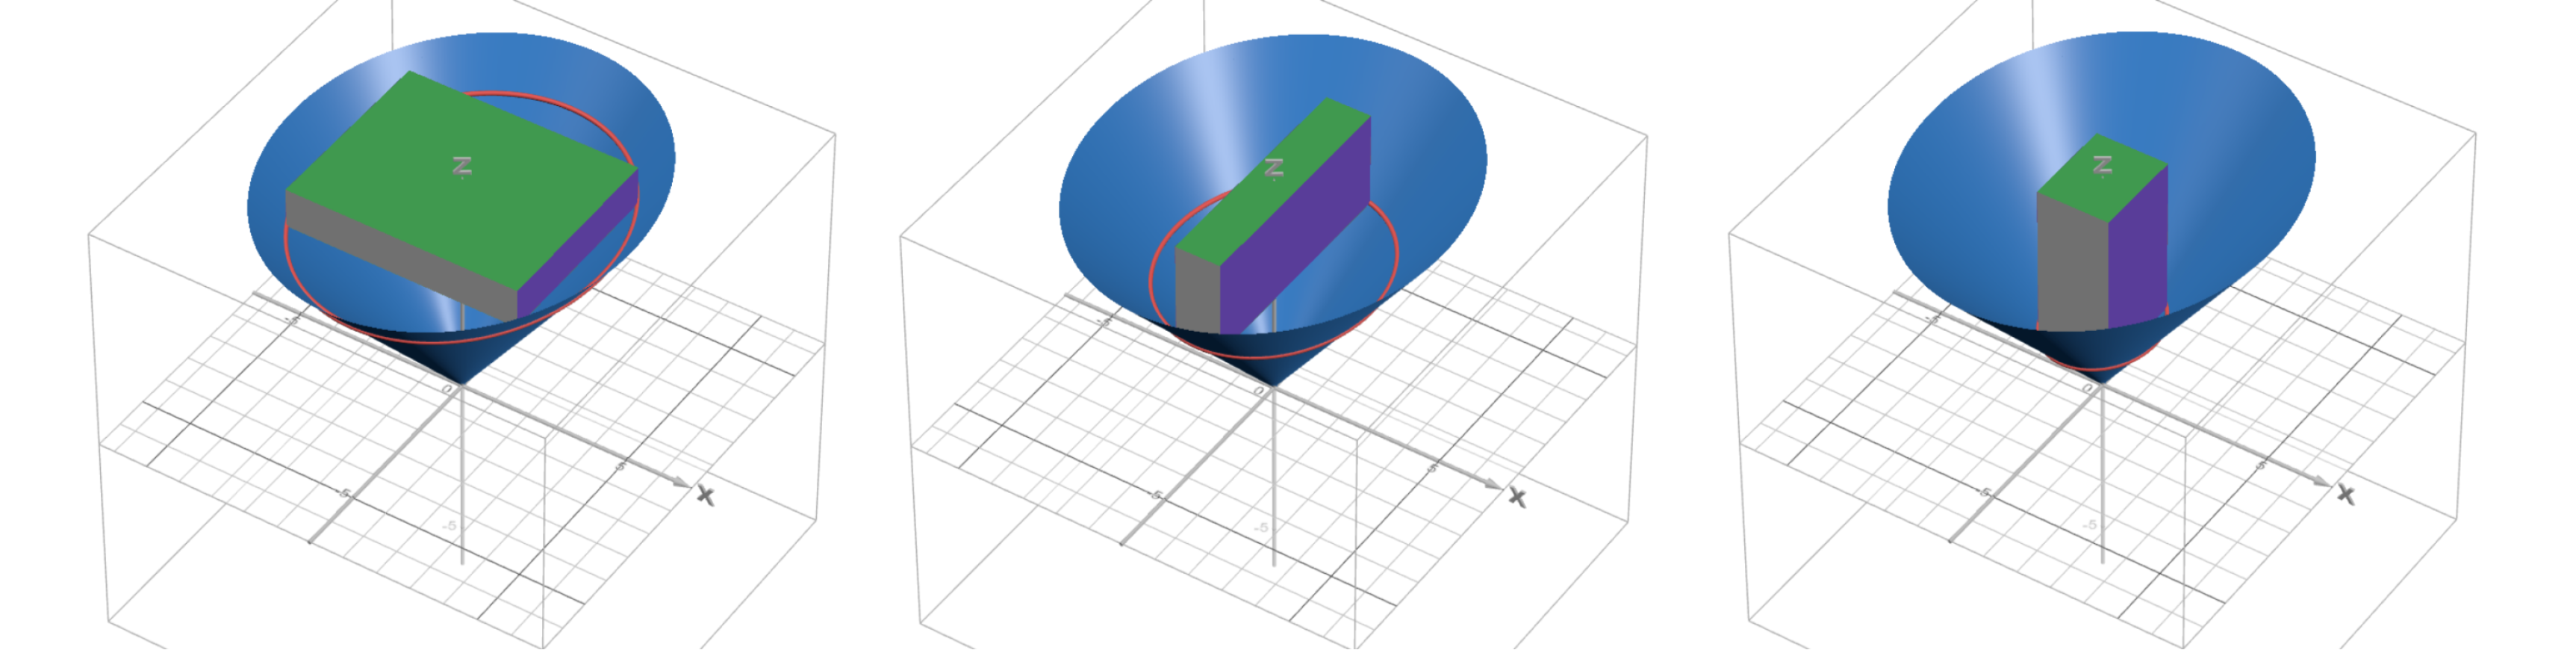
\includegraphics[width=1\textwidth]{ex.png}
    \end{center}

\caption{Примеры призмы, вписанной в конус}
\end{figure}





\subsection{Объём призмы, вписанной в конус}
Объем призмы вычисляется по формуле
$$V = S_{\text{осн}} \cdot h,$$
где $S_{\text{осн}}$ - площадь основания, $h$ - высота призмы.\\
Расположим вершину конуса в начале координат. Тогда уравнение конической поверхности примет канонический вид:
$$
\frac{x^2}{a^2} + \frac{y^2}{b^2} = \frac{z^2}{c^2}
$$

Нас интересует не вся коническая поверхность, а только ее верхняя часть, ограниченная плоскостью $z = H$.
$$
\frac{x^2}{A^2} + \frac{y^2}{B^2} = \frac{z^2}{H^2}, \; 0 \leq z \leq H
$$
Призма вписана в конус. Это значит, что одно её основание лежит в плоскости $z = H$. Другое - на некоторой высоте, в плоскости $z = z_0$, и вершины этого основания лежат на образующих конуса. $z_0$ - это варьируемый параметр, ненулевое расстояние от начала координат до нижнего основания. Тогда высота полученнной призмы есть $(H - z_0)$.\\

Рассмторим сечение конуса плоскостью $z = z_0, \; 0 < z_0 < H$. В сечении ожидаемо получится эллипс:
$$
\frac{x^2}{A^2 \cdot \frac{z_0^2}{H^2}} + \frac{y^2}{B^2 \cdot \frac{z_0^2}{H^2}} = 1
$$
Введем обозначения полуосей эллипса, полученного в результате такого сечения:
$$
a(z_0) =  \frac{A}{H} z_0, \; b(z_0) =  \frac{B}{H} z_0,
$$
Уравнение эллипса приняло более компактный вид:
$$
\frac{x^2}{a(z_0)^2} + \frac{y^2}{b(z_0)^2} = 1
$$
Точки нижнего основания призмы лежат на этом эллипсе. Известно, что основание призмы представляет собой прямоугольник, пересечение диагоналей которого лежит в центре эллипса. Если одна из вершин задается точкой $(x_0, y_0)$, то оставшиеся три вершины задаются точками: $(-x_0, y_0)$, $(-x_0, -y_0)$, $(x_0, -y_0)$.
\begin{figure}[H]
    \begin{center}
        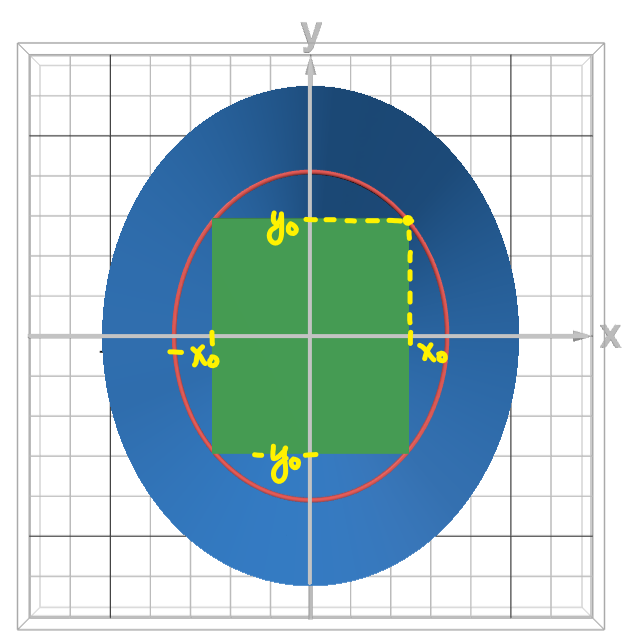
\includegraphics[width=.5\textwidth]{up.png}
    \end{center}
\caption{Вид сверху}
\end{figure}
В силу симметри примем значения $x_0$ и $y_0$ строго положительными. Тогда длины сторон такого прямоугольника равны $2x_0$ и $2y_0$, а площадь $S_{\text{осн}} = 4x_0y_0$.

Вспомним, что вершины прямоугольника принадлежат эллипсу. Тогда при фиксации варьируемого параметра $x_0, 0 < x_0 < a(z_0)$ получим единственное значение $y_0$. Найдем его:
$$
\frac{x_0^2}{a(z_0)^2} + \frac{y_0^2}{b(z_0)^2} = 1
$$
$$
y_0^2 = b(z_0)^2 \frac{a(z_0)^2 - x_0^2}{a(z_0)^2}
$$
$$
y_0 = \frac{B}{A} \sqrt{\frac{A^2}{H^2} z_0^2 - x_0^2} 
$$

Таким образом, запишем выражение для объема призмы, вписанной в конус.
$$
V = S_{\text{осн}} \cdot h = 4x_0y_0(H-z_0)
$$
$$
V(z_0, x_0) = 4x_0\frac{B}{A} \sqrt{\frac{A^2}{H^2} z_0^2 - x_0^2} (H - z_0)
$$
Или, если ввести обозначение для корня:
$$
V(z_0, x_0) = 4\frac{B}{A} x_0 K (H - z_0), \; K = \sqrt{\frac{A^2}{H^2} z_0^2 - x_0^2}
$$
Область определения: 
$$
0 < z_0 < H, \; 0 < x_0 < \frac{A}{H}z_0
$$




\subsection{Поиск максимума функции}
Максимум функции достигается в точке максимума. По необходимуму условию экстремума точки экстремума нужно искать среди критических точек функции. Для нахождения критических точек возьмем частные производные функции объёма призмы:
$$
\frac{\partial V}{\partial z_0} = 4\frac{B}{A} x_0 
\left( 
\frac{2\frac{A^2}{H^2}z_0}{2K} (H-z_0) - K
\right) 
$$

$$
\frac{\partial V}{\partial x_0} = 4\frac{B}{A} (H-z_0) 
\left( 
K - x_0 \frac{2x_0}{2K}
\right) 
$$
Эти производные существуют и не обращаются в бексонечность на всей области определения:
$$
0 < z_0 < H, \; 0 < x_0 < \frac{A}{H}z_0
$$
Поэтому задача по нахождению критических точек сводится к нахождению стационарных точек. Найдем такие точки, в которых обе производные равны нулю одновременно. Начнем рассмотрение с частной производной по $x_0$.
$$
4\frac{B}{A} (H-z_0) 
\left( 
K - x_0 \frac{2x_0}{2K}
\right) = 0
$$
$$
(H-z_0) 
\left( 
K^2 - x_0^2
\right) = 0
$$
$$
(H-z_0) 
\left( 
\frac{A^2}{H^2} z_0^2 - x_0^2 - x_0^2
\right) = 0
$$
$$
z_0 = H - \text{не входит в ОДЗ}
$$
$$
x_0 = - \frac{1}{\sqrt{2}}\frac{A}{H}z_0 - \text{не входит в ОДЗ}
$$
$$
x_0 = \frac{1}{\sqrt{2}}\frac{A}{H}z_0
$$
Подставим найденное значение $x_0$ в частную производную по $z_0$:
$$
4\frac{B}{A} x_0 
\left( 
\frac{2\frac{A^2}{H^2}z_0}{2K} (H-z_0) - K
\right) = 0
$$
$$
x_0 
\left( 
\frac{A^2}{H^2}z_0 (H-z_0) - K^2
\right) = 0
$$
$$
x_0 
\left( 
\frac{A^2}{H^2}z_0 (H-z_0) - \frac{A^2}{H^2} z_0^2 + x_0^2
\right) = 0
$$
$$
\frac{1}{\sqrt{2}}\frac{A}{H}z_0 
\left( 
\frac{A^2}{H^2}z_0 (H-z_0) - \frac{A^2}{H^2} z_0^2 + \frac{1}{2}\frac{A^2}{H^2}z_0^2
\right) = 0
$$
$$
z_0^2
\left( 
H-z_0 - z_0 + \frac{1}{2}z_0
\right) = 0
$$
$$
z_0^2
\left( 
H - \frac{3}{2}z_0
\right) = 0
$$
$$
z_0 = 0 - \text{не входит в ОДЗ}
$$
$$
z_0 = \frac{2}{3}H
$$
$$
x_0 = \frac{1}{\sqrt{2}}\frac{A}{H} z_0 = \frac{\sqrt{2}}{3}A
$$
Нашли единственную стационарную точку для нашей ОДЗ. Проверим, что она является точкой максимума.\\
Воспользуемся достаточным условием экстремума функции двух переменных для стационораной точки. Для начала вычилим значения вторых частных производных функции $V$ в точке исследуемой точке $M(z_0 = \frac{2}{3}H; \; x_0 = \frac{\sqrt{2}}{3}A)$.
$$
\frac{\partial V}{\partial z_0} = 4\frac{B}{A} x_0 
\left( 
\frac{A^2}{H^2}z_0 (H-z_0) - K^2
\right) \frac{1}{K}
$$

$$
\frac{\partial V}{\partial x_0} = 4\frac{B}{A} (H-z_0) 
\left( 
K^2 - x_0^2
\right) \frac{1}{K}
$$
$$
K_M = \sqrt{\frac{A^2}{H^2} \frac{4}{9}H^2 - \frac{2}{9}A^2} = \frac{\sqrt{2}A}{3} = x_{0_M}
$$
$$
(H-z_0)_M = H - \frac{2}{3}H = \frac{1}{3}H
$$
Так как ислледуемая точка $M$ является стационарной,
$$
\left( 
\frac{A^2}{H^2}z_0 (H-z_0) - K^2
\right)_M = 0 \text{ и }
\left( 
K^2 - x_0^2
\right)_M = 0
$$
то вид вторых частных производных $V$ в точке $M$ упрощается, останутся только те слагаемые, где взяты производные от этих "скобочек".
$$
\frac{\partial^2 V}{\partial z_0^2} (M) = 4\frac{B}{A} x_0 
\left( 
\frac{A^2}{H^2}z_0H - \frac{A^2}{H^2}z_0^2 - \frac{A^2}{H^2} z_0^2 + x_0^2
\right)'_{z_0} \frac{1}{K} = 
$$
$$
= 4\frac{BA}{H^2} x_0 
\left( 
-4z_0 + H
\right)\frac{1}{K} =  
4\frac{BA}{H^2} 
\left( 
-\frac{8H}{3} + H
\right) = 
$$
$$
= -\frac{20}{3}\frac{AB}{H} = \cal A
$$


$$
\frac{\partial^2 V}{\partial x_0^2} = 4\frac{B}{A} (H-z_0) 
\left( 
\frac{A^2}{H^2}z_0^2 - 2x_0^2
\right)'_{x_0} \frac{1}{K} = 
$$
$$
= 4\frac{B}{A} \frac{H}{3} 
\left( 
 - 4x_0
\right) \frac{1}{K} = -\frac{16}{3}\frac{BH}{A} = \cal C
$$


$$
\frac{\partial^2 V}{\partial x_0 \partial z_0} = 4\frac{B}{A} (H-z_0) 
\left( 
\frac{A^2}{H^2}z_0^2 - 2x_0^2
\right)'_{z_0} \frac{1}{K} = 
$$
$$
= 4\frac{B}{A} (H-z_0) 
\left( 
2\frac{A^2}{H^2}z_0
\right) \frac{1}{K} = 
4\frac{B}{A} \frac{H}{3}
2\frac{A^2}{H^2} \frac{2H}{3}
 \frac{3}{\sqrt{2}A} =
$$
$$
= \frac{16}{3\sqrt{2}}B = \cal B
$$
$$
\cal D = \cal A \cal C - \cal B ^{\text{2}} = 
$$
$$
= -\frac{20}{3}\frac{AB}{H} \cdot -\frac{16}{3}\frac{BH}{A} - \frac{16 \cdot 16}{18}B^2 = \frac{20 \cdot 16 \cdot 2}{18}B^2 - \frac{16 \cdot 16}{18}B^2
$$
Так как $\cal D$ $> 0$ и $\cal A$ $< 0$, то по достаточному условию экстремума функции двух переменных для стационораной точки точка $M(z_0 = \frac{2}{3}H; \; x_0 = \frac{\sqrt{2}}{3}A)$ является точкой максимума.

\subsection{Конечный результат}
Высота полученной призмы:
$$
h = H - z_0 = \frac{H}{3}
$$
Стороны основания:
$$
a = 2x_0 = \frac{2\sqrt{2}}{3}A
$$
$$
b = 2y_0 = \frac{B}{A} K_M = 2 \frac{B}{A} \frac{\sqrt{2}}{3}A = \frac{2 \sqrt{2}}{3}B
$$
Максимальный объем призмы, вписанной в конус:
$$
V = a \cdot b \cdot h = \frac{8}{27}ABH
$$

\begin{figure}[H]
    \begin{center}
        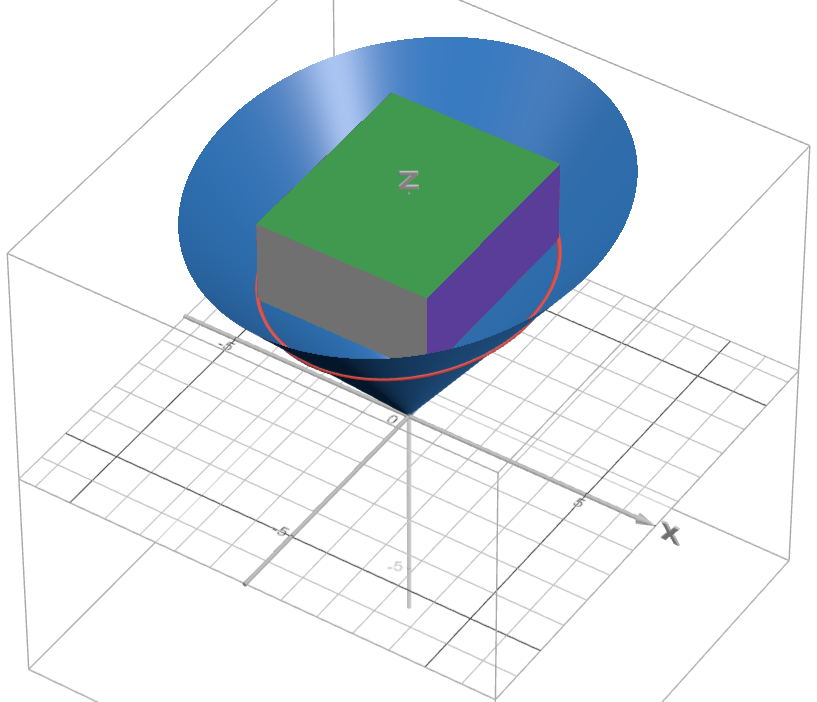
\includegraphics[width=.5\textwidth]{res.png}
    \end{center}
\caption{Итоговый результат. \href{https://www.desmos.com/3d/88d50f8402}{[интерактивный пример в редакторе Desmos 3D]}}
\end{figure}
\newpage
\section*{Задание 2. Интегралы Пуассона и Френеля}
В задачах физики и дифракционной оптики возникают интегралы вида:
\begin{equation*}
\begin{aligned}
\int\limits e^{-x^2}dx, \int\limits \frac{\sin{t}}{\sqrt{t}} dt, \int\limits \frac{\cos{t}}{\sqrt{t}} dt
\end{aligned}
\end{equation*}

которые являются специальными функциями (т.е. "неберущимися" интегралами). Однако, переход
к "многомерным" интегралам позволяет вычислить по крайней мере:

\begin{equation*}
\begin{aligned}
\int\limits_0^{\infty} e^{-x^2}dx, \int\limits_0^{\infty} \frac{\sin{t}}{\sqrt{t}} dt, \int\limits_0^{\infty} \frac{\cos{t}}{\sqrt{t}} dt
\end{aligned}
\end{equation*}

где $\Phi(z) = \int\limits_0^{z} e^{-x^2}dx$ - функция ошибок, $\Phi_{S}(z) = \int\limits_0^{z} \frac{\sin{t}}{\sqrt{t}} dt$ и $\Phi_{C}(z) = \int\limits_0^{z} \frac{\cos{t}}{\sqrt{t}} dt$ - интегралы Френеля.

\subsection*{Постановка задачи}

Вычислите интеграл $K$:
\begin{equation*}
\begin{aligned}
\int\limits_0^{\infty} \frac{\sin(3t + \frac{3\pi}{2})}{\sqrt{t}} dt
\end{aligned}
\end{equation*}

\subsection*{Решение}

Для начала попробуем вычислить интеграл $\int\limits_0^{\infty} e^{-x^2}dx = I$. Заметим, что $I = \int\limits_0^{\infty} e^{-x^2}dx =  \int\limits_0^{\infty} e^{-y^2}dy$, то есть возможен переход к двукратному интегралу:
\begin{equation*}
\begin{aligned}
I^2 = \int\limits_0^{\infty} e^{-x^2}dx \int\limits_0^{\infty} e^{-y^2}dy
\end{aligned}
\end{equation*}
Вычислим его с переходоим в полярные координаты:
\begin{equation*}
\begin{aligned}
\begin{cases}
x = \rho \cdot \cos{\phi}\\
y= \rho \cdot \sin{\phi}
\end{cases}
J \text{ - Якобиан, } J = \rho
\end{aligned}
\end{equation*}

Пределы интегрирования в таком случае находятся как:
\begin{equation*}
\begin{aligned}
\begin{cases}
\rho \cdot \cos{\phi} > 0 \\
 \rho \cdot \sin{\phi} >0 \\
 \rho > 0 \\
  \phi \in \left[0; 2\pi\right)
\end{cases} \Rightarrow
\begin{cases}
 \cos{\phi} > 0 \\
  \sin{\phi} >0 \\
  \rho > 0 \\
\end{cases} \Rightarrow
\begin{cases}
\phi \in \left[0; \frac{\pi}{2}\right]\\
  \rho > 0 \\
  \end{cases}
\end{aligned}
\end{equation*}

Таким образом:

\begin{equation*}
\begin{aligned}
I^2 &= \int\limits_0^{\infty} e^{-x^2}dx \int\limits_0^{\infty} e^{-y^2}dy = \int\limits_0^{\frac{\pi}{2}} d\phi \int\limits_0^{\infty} e^{-\rho^2 \cos^2{\phi}}\cdot e^{-\rho^2 \sin^2{\phi}}  \cdot \rho d\rho \\
&= \frac{1}{2}\int\limits_0^{\frac{\pi}{2}} d\phi \int\limits_0^{\infty} e^{-\rho^2}  \cdot  d\rho^2 = -\frac{1}{2}\int\limits_0^{\frac{\pi}{2}} \left. e^{-\rho^2} \right|_0^{\infty} d\phi\\
& = \frac{1}{2}\int\limits_0^{\frac{\pi}{2}} d\phi = \frac{\pi}{4} \Rightarrow I= \sqrt{\frac{\pi}{2}}\\
\end{aligned}
\end{equation*}

Далее вычислим интеграл $\int\limits_0^{\infty} \frac{\cos{t}}{\sqrt{t}} dt = J$. Сначала докажем полезное равенство:

\begin{equation*}
\begin{aligned}
\frac{1}{\sqrt{t}} &= \frac{2}{\sqrt{\pi}} \int\limits_0^{\infty} e^{-u^2 t}du \\
\frac{1}{\sqrt{t}} &= \frac{2}{\sqrt{\pi t}} \int\limits_0^{\infty} e^{-u^2 \sqrt{t}^2}du\sqrt{t} \\
\frac{1}{\sqrt{t}} &= \frac{2}{\sqrt{\pi t}} \frac{\sqrt{\pi}}{2}
\end{aligned}
\end{equation*}

С его помощью решим упомянутый интеграл $J$:
\begin{equation*}
\begin{aligned}
\int\limits_0^{\infty} \frac{\cos{t}}{\sqrt{t}} dt &= \int\limits_0^{\infty} \cos{t} \cdot \frac{2}{\pi} \int\limits_0^{\infty} e^{-u^2 t}du dt
\end{aligned}
\end{equation*}
При этом сменим порядок интегрирования ( в силу несобственности интеграла смена порядка требует обоснованя, но в данном случае она разрешена):
\begin{equation*}
\begin{aligned}
\frac{2}{\sqrt{\pi}} \int\limits_0^{\infty} du  \int\limits_0^{\infty} \cos{t} \cdot  e^{-u^2 t} dt \\
\int\limits_0^{\infty} \cos{t} \cdot  e^{-u^2 t} dt &= |\text{По частям}| =\\
\left. \sin{t} \cdot e^{-u^2 t} \right|_0^{\infty} + u^2 \cdot \int\limits_0^{\infty} \sin{t} \cdot  e^{-u^2 t} dt &=\\
 \left.\sin{t} \cdot e^{-u^2 t} \right|_0^{\infty} + u^2 \left( \left. -\cos{t} \right|_0^{\infty} e^{-u^2 t} - u^2\int\limits_0^{\infty} \cos{t} \cdot  e^{-u^2 t} dt \right) & \Rightarrow\\
\int\limits_0^{\infty} \cos{t} \cdot  e^{-u^2 t} dt = \left. \sin{t} \cdot e^{-u^2 t} \right|_0^{\infty} + \left. u^2 \cdot \cos{t} e^{-u^2 t} \right|_0^{\infty} - u^4 \int\limits_0^{\infty} \cos{t}\cdot  e^{-u^2 t} dt \\
\int\limits_0^{\infty} \cos{t}\cdot  e^{-u^2 t} dt =\left. \frac{e^{-u^2 t}\cdot \left(\sin{t} + u^2 \cos{t} \right)}{1 + u^4} \right|_0^{\infty} = \frac{u^2}{1+u^2} \Rightarrow \\
\frac{2}{\sqrt{\pi}} \int\limits_0^{\infty} du  \int\limits_0^{\infty} \cos{t}\cdot  e^{-u^2 t} dt = \frac{2}{\sqrt{\pi}} \int\limits_0^{\infty} \frac{u^2}{1+u^4} du 
\end{aligned}
\end{equation*}

\begin{equation*}
\begin{aligned}
\frac{2}{\sqrt{\pi}} \int\limits_0^{\infty} \frac{u^2}{1+u^4} du = \frac{2}{\sqrt{\pi}} \int\limits_0^{\infty} \frac{u^2}{ (u^2-\sqrt{2}u+1) (u^2+\sqrt{2}+1) } du = |\text{Инт. Дроб.-Рац.}| =\\
\frac{2}{\sqrt{\pi}} \int\limits_0^{\infty} \frac{u}{ 2\sqrt{2}(u^2-\sqrt{2}u+1)} - \frac{u}{2\sqrt{2}(u^2+\sqrt{2}+1) } du =\\
\frac{2}{\sqrt{\pi}} \left( \frac{1}{2\sqrt{2}}\cdot \int\limits_0^{\infty} \frac{u}{(u^2-\sqrt{2}u+1)} du - \frac{1}{2\sqrt{2}}\cdot \int\limits_0^{\infty} \frac{u}{(u^2+\sqrt{2}u+1)} du \right) =\\
\frac{2}{\sqrt{\pi}} \left( \frac{1}{2\sqrt{2}} (1) - \frac{1}{2\sqrt{2}} (2) \right)
\end{aligned}
\end{equation*}

\begin{equation*}
\begin{aligned}
(1) = \int\limits_0^{\infty} \frac{u}{(u^2-\sqrt{2}u+1)} du = |u = \frac{1}{2}(2u-\sqrt{2})+\frac{1}{\sqrt{2}}| \\
(1) = \frac{1}{2} \int\limits_0^{\infty} \frac{2u-\sqrt{2}}{(u^2-\sqrt{2}u+1)} du + \int\limits_0^{\infty} \frac{1}{\sqrt{2}(u^2-\sqrt{2}u+1)} du =\\
\frac{1}{2} \int\limits_0^{\infty} \frac{1}{(u^2-\sqrt{2}u+1)} d(u^2 -\sqrt{2}u+1) + \int\limits_0^{\infty} \frac{1}{\sqrt{2}}\frac{1}{(u-\frac{1}{\sqrt{2}})^2+\frac{1}{2}} du = \\
\left. \frac{1}{2}\cdot \ln{\left|u^2-\sqrt{2}u+1\right|} \right|_0^{\infty} + \left. \frac{1}{\sqrt{2}}\cdot \sqrt{2}\cdot \arctan(\sqrt{2}u-1) \right|_0^{\infty}
\end{aligned}
\end{equation*}
Аналогично:
\begin{equation*}
\begin{aligned}
(2) = \left. \frac{1}{2}\cdot \ln{\left|u^2+\sqrt{2}u+1\right|} \right|_0^{\infty} - \left. \frac{1}{\sqrt{2}}\cdot \sqrt{2}\cdot \arctan(\sqrt{2}u+1) \right|_0^{\infty}
\end{aligned}
\end{equation*}
Следовательно:

\begin{equation*}
\begin{aligned}
\frac{2}{\sqrt{\pi}} \int\limits_0^{\infty} \frac{u^2}{1+u^4} du = \frac{2}{\sqrt{\pi}} \left( \frac{1}{2\sqrt{2}} (1) - \frac{1}{2\sqrt{2}} (2) \right) = \\
\left. \frac{2}{2\sqrt{2}\sqrt{\pi}} \left( \frac{1}{2}  \ln{\left|\frac{u^2-\sqrt{2}u+1}{u^2-\sqrt{2}u+1}\right|} +   \arctan(\sqrt{2}u+1) +  \arctan(\sqrt{2}u-1)  \right) \right|_0^{\infty} = \\
\frac{2}{2\sqrt{2} \sqrt{\pi}}\cdot \left(\frac{\pi}{2} + \frac{\pi}{2} - \frac{\pi}{4} - \left(-\frac{\pi}{4}\right) \right) = \sqrt{\frac{\pi}{2}}
\end{aligned}
\end{equation*}
То есть:
\begin{equation*}
\begin{aligned}
J = \int\limits_0^{\infty} \frac{\cos{t}}{\sqrt{t}} dt = \sqrt{\frac{\pi}{2}}
\end{aligned}
\end{equation*}

Наконец вычислим искомый интеграл $K$:
\begin{equation*}
\begin{aligned}
K = \int\limits_0^{\infty} \frac{\sin(3t + \frac{3\pi}{2})}{\sqrt{t}} dt = -\frac{\sqrt{3}}{3}\int\limits_0^{\infty} \frac{\cos{3t}}{\sqrt{3t}} d (3t) = -\frac{\sqrt{3}}{3}\cdot \sqrt{\frac{\pi}{2}} = -\sqrt{\frac{\pi}{6}}
\end{aligned}
\end{equation*}

Используя замену переменной и сводя интегралы к $J$ вычислим также:
\begin{equation*}
\begin{aligned}
\int_0^{\infty} \cos{x}^2 dx = \int_0^{\infty} \frac{\cos{x}^2}{2 \sqrt{x^2}} d x^2 = \frac{1}{2}\cdot \sqrt{\frac{\pi}{2}} = \frac{\sqrt{\pi}}{2\sqrt{2}}
\end{aligned}
\end{equation*}

\begin{equation*}
\begin{aligned}
\int_0^{\infty} \cos{\frac{\pi x^2}{2}} dx = \frac{2}{2\pi}\cdot \frac{\sqrt{\pi}}{\sqrt{2}}	\int_0^{\infty} \frac{\cos{\frac{\pi x^2}{2}}}{\sqrt{\frac{\pi x^2}{2}}} d \frac{\pi x^2}{2} = \frac{1}{\sqrt{2\pi}}\cdot \sqrt{\frac{\pi}{2}} = \frac{1}{2}
\end{aligned}
\end{equation*}

Рассмотрим графики исследуемых интегралов и их подынтегральных функций:

\fboxsep=0mm%padding thickness
\fboxrule=2pt%border thickness
\begin{figure}[H]
\centering
\begin{minipage}[t]{.4\textwidth}
\begin{figure}[H]
  \centering
  \fbox{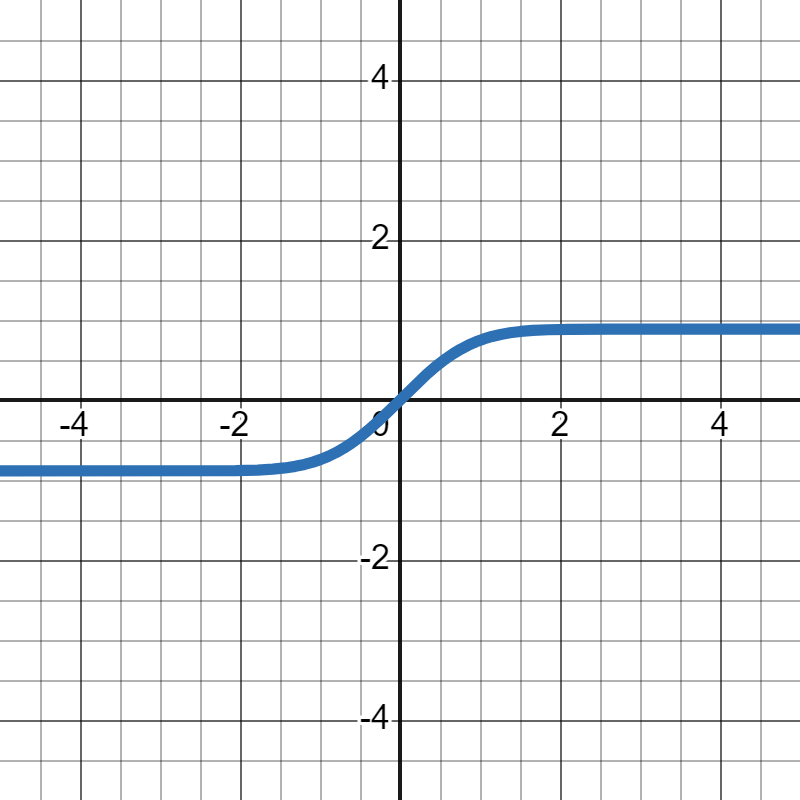
\includegraphics[width=1\textwidth]{err}}%
  \caption{График функции ошибок $\Phi(z) = \int\limits_0^{z} e^{-x^2}dx$}
  \label{fig:err_int}
  \end{figure}%
\end{minipage}\hspace{10pt}%
\begin{minipage}[t]{.4\textwidth}%
\begin{figure}[H]
  \centering
  \fbox{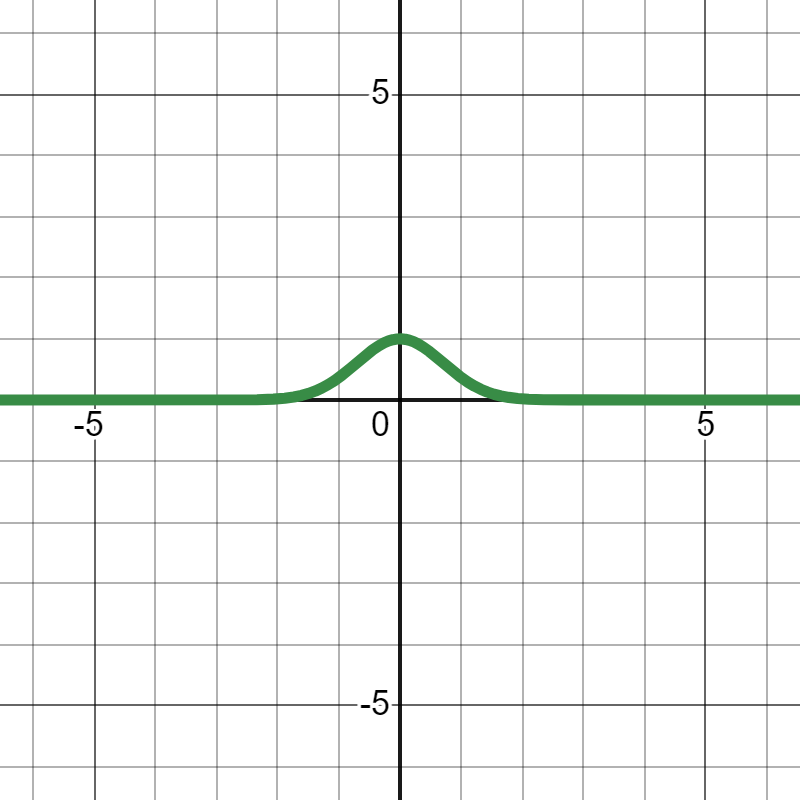
\includegraphics[width=1\textwidth]{err_fun}}%
  \caption{График подынтегральной фукнции для функции ошибок $y =  e^{-x^2}$}
  \label{fig:err_fun}
    \end{figure}
\end{minipage}
\end{figure}

\begin{figure}[H]
\centering
\begin{minipage}[t]{.4\textwidth}
\begin{figure}[H]
  \centering
  \fbox{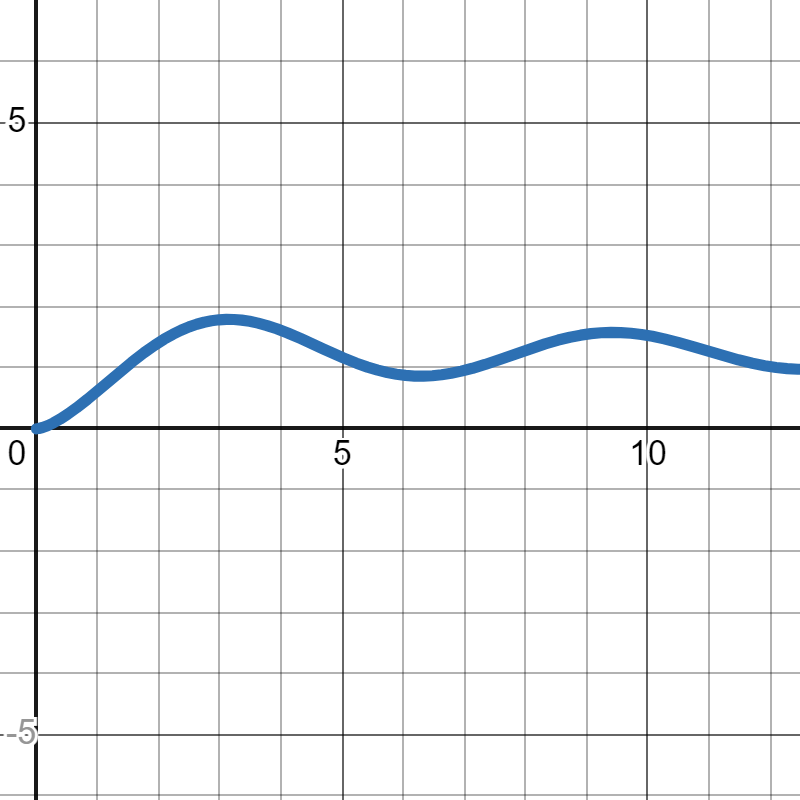
\includegraphics[width=1\textwidth]{fren1}}%
  \caption{График интеграла Френеля $\Phi_{S}(z) = \int\limits_0^{z} \frac{\sin{t}}{\sqrt{t}} dt$}
  \label{fig:fren1_int}
  \end{figure}%
\end{minipage}\hspace{10pt}%
\begin{minipage}[t]{.4\textwidth}%
\begin{figure}[H]
  \centering
  \fbox{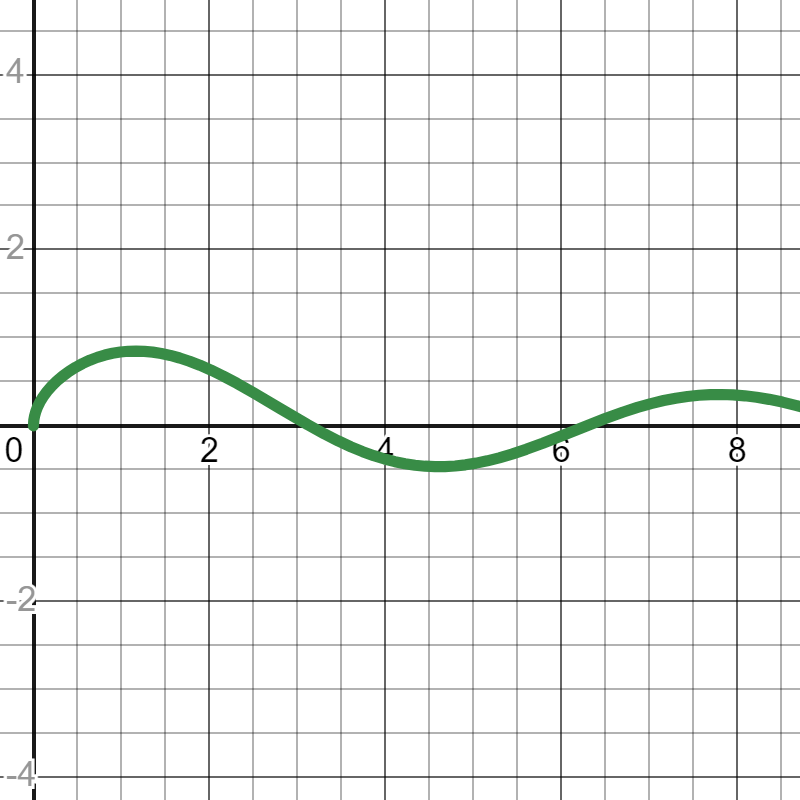
\includegraphics[width=1\textwidth]{fren1_fun}}%
  \caption{График подынтегральной функции для фукнции Френеля $y =  \frac{\sin{x}}{\sqrt{x}}$}
  \label{fig:fren1_fun}
    \end{figure}
\end{minipage}
\end{figure}

\begin{figure}[H]
\centering
\begin{minipage}[t]{.4\textwidth}
\begin{figure}[H]
  \centering
  \fbox{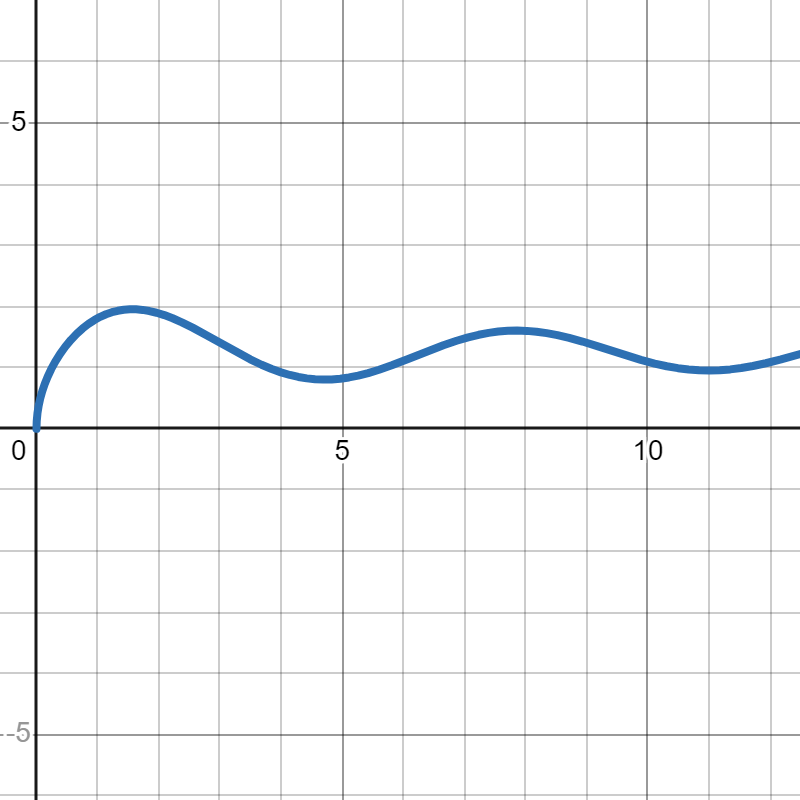
\includegraphics[width=1\textwidth]{fren2}}%
  \caption{График интеграла Френеля $\Phi_{S}(z) = \int\limits_0^{z} \frac{\cos{t}}{\sqrt{t}} dt$}
  \label{fig:fren2_int}
  \end{figure}%
\end{minipage}\hspace{10pt}%
\begin{minipage}[t]{.4\textwidth}%
\begin{figure}[H]
  \centering
  \fbox{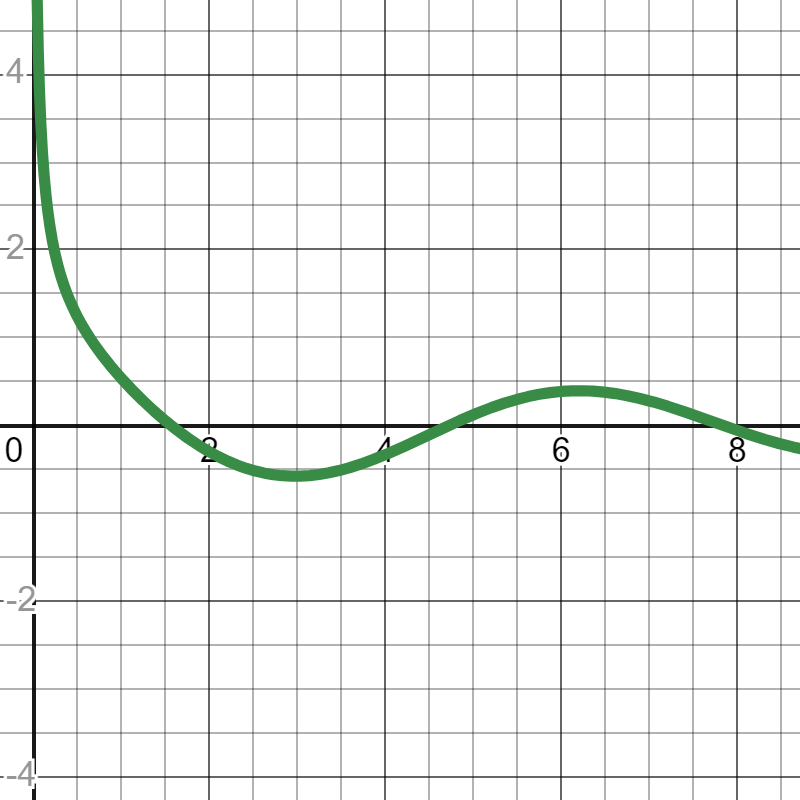
\includegraphics[width=1\textwidth]{fren2_fun}}%
  \caption{График подынтегральной функции для фукнции Френеля $y =  \frac{\cos{x}}{\sqrt{x}}$}
  \label{fig:fren2_fun}
    \end{figure}
\end{minipage}
\end{figure}

\newpage
\section*{Задание 3. Потенциал векторного поля}
Дано: векторное поле $\vec{H}$
\begin{equation*}
    \vec{H} = (e^x;-e^{y}) = e^x\cdot \overline{i}+(-e^y)\cdot\overline{j}
\end{equation*}
Решение:
\\ \\
1) Убедитесь, что данное векторное поле потенциально.

Чтобы доказать, что поле потенциально достаточно одного критерия. Векторное поле потенциально, если оно является градиентом некоторого скалярного поля. 
Необходимо и достаточно следующее:
\begin{equation*}
    rot(\vec{F}) = \overline{\nabla}\text{ x }\vec{F} = 
    \begin{vmatrix}
        \overline{i}&\overline{j}&\overline{k}\\
        \pdv{}{x}&\pdv{}{y}&\pdv{}{z}\\
        P&Q&R\\
    \end{vmatrix}
    = 0
\end{equation*}
\begin{equation*}
    rot(\vec{H}) = \overline{\nabla}\text{ x }\vec{H} = 
    \begin{vmatrix}
        \overline{i}&\overline{j}&\overline{k}\\
        \pdv{}{x}&\pdv{}{y}&\pdv{}{z}\\
        P&Q&R\\
    \end{vmatrix}
    = \overline{i}(0-0) + \overline{j}(0-0) + \overline{k}(0-0)
    = 0
\end{equation*}
Поле потенциально (безвихриво).
\\
\\
2) Найдите уравнения векторных линий. Изобразите векторные линии на рисунке.

Векторные линии можно найти следующим способом:
\begin{equation*}
    tg\alpha = y' = \frac{Q}{P}
\end{equation*}
\begin{equation*}
    y' = \frac{-e^y}{e^x}
\end{equation*}
После решения ДУ, получили уравнение векторных линий:
\begin{equation*}
    y = ln\left(\frac{e^x}{Ce^x-1}\right),\ C\in \mathbb{R}
\end{equation*}
Векторные линии поля на графике:
\begin{center}
    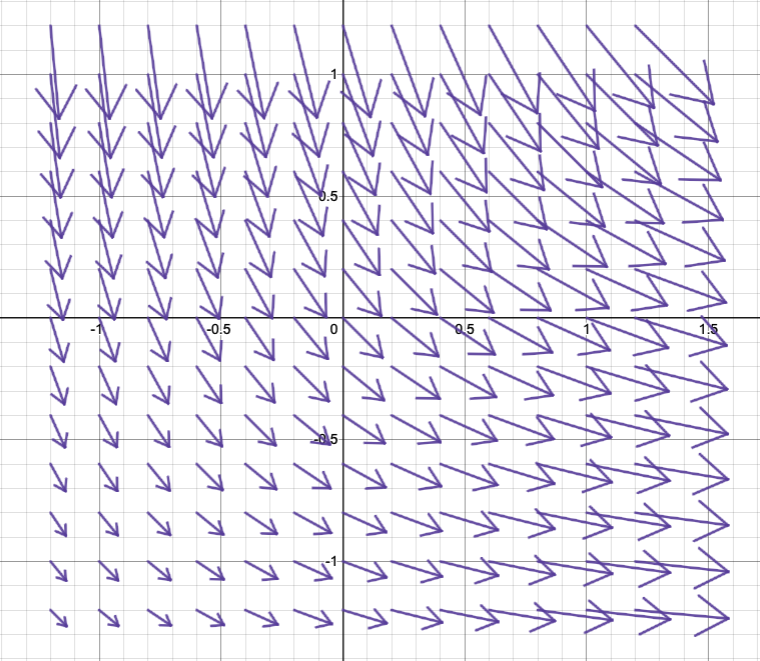
\includegraphics[width=.5\textwidth]{vecLin.png}
\end{center}
3) Найдите потенциал поля при помощи криволинейного интеграла.
\begin{equation*}
    \mathbb{U}(x, y) = \int_{AB}Pdx+Qdy = \int_{x_0}^{x}P(x, y)dx +\int_{y_0}^{y}Q(x, y)dx
\end{equation*}
\begin{equation*}
    \mathbb{U}(x, y) = \int_{x_0}^{x}e^xdx -\int_{y_0}^{y}e^ydx = e^x-e^y-e^{x_0}+e^{y_0}
\end{equation*}
Проверка:
\begin{equation*}
    grad(\mathbb{U}) = \vec{H} = \pdv{\mathbb{U}}{x} + \pdv{\mathbb{U}}{y}
\end{equation*}
\begin{equation*}
    \pdv{\mathbb{U}}{x} = e^x
\end{equation*}
\begin{equation*}
    \pdv{\mathbb{U}}{y} = -e^y
\end{equation*}
\begin{equation*}
    grad(\mathbb{U}) = \vec{H} = e^x -e^y
\end{equation*}
\\
4) Найдите уравнения линий уровня потенциала (эквипотенциальных линий). Изобразите
линии уровня потенциала.

Существует такая $f$, что:
\begin{equation*}
    \nabla f = \vec{H}
\end{equation*}
Тогда:
\begin{equation*}
    \pdv{f(x,y)}{x} = e^x;\ f(x,y) = \int e^xdx = e^x + C(y)
\end{equation*}
\begin{equation*}
    \pdv{f(x,y)}{x} = -e^y;\ f(x,y) = \int -e^ydx = -e^y + C_1
\end{equation*}
\begin{equation*}
    f(x, y) = e^x - e^y + C_1
\end{equation*}
Линии уровня:
\begin{equation*}
    f(x, y) = C_2
\end{equation*}
\begin{equation*}
    e^x - e^y = C\
\end{equation*}
\begin{equation*}
    y = ln(e^x-C)
\end{equation*}
Линии уровня потенциала:
\begin{center}
    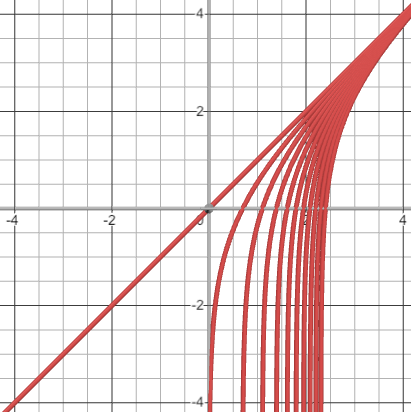
\includegraphics[width=.5\textwidth]{linU.png}
\end{center}
5) Докажите ортогональность найденных векторных линий поля и линий уровня потенциала.
Проиллюстрируйте ортогональность на графике.

Докажем ортогональность для
\begin{equation*}
    y_u = ln(e^x-C_1); \ y_v = ln\left(\frac{e^x}{C_2e^x-1}\right)
\end{equation*}
Зафиксируем точку $C = C_1 = C_2$ и найдём производные:
\begin{equation*}
    y_u' = \frac{e^x}{e^x-C}; \ y_v' = -\frac{1}{Ce^x-1}
\end{equation*}
Произведение производных в точне пересечения, которую определяет в первую очередь параметр C, должно быть равно -1. Покажем общую формулу, где предположим, что $x=x_0$
\begin{equation*}
    y_u'\cdot y_v' =(\frac{e^{x_0}}{e^{x_0}-C})\cdot (-\frac{1}{Ce^{x_0}-1}) = - \frac{e^{x_0}}{Ce^{2x_0}-e^{x_0}-C^2e^{x_0}+C}
\end{equation*}
Пусть фиксированная C = 1, тогда точка пересечения:
\begin{equation*}
    e^x-e^{ln(\frac{e^x}{e^x-1})} = 1
\end{equation*}
\begin{equation*}
    x= ln\left(\frac{3+\sqrt{5}}{2}\right)
\end{equation*}
Подставим эту точку:
\begin{equation*}
    y_u'\cdot y_v' = - \frac{e^{ln\left(\frac{3+\sqrt{5}}{2}\right)}}{e^{2ln\left(\frac{3+\sqrt{5}}{2}\right)}-e^{ln\left(\frac{3+\sqrt{5}}{2}\right)}-e^{ln\left(\frac{3+\sqrt{5}}{2}\right)}+1} = -1
\end{equation*}
Проиллюстрируем ортогональность на графике.
\begin{center}
    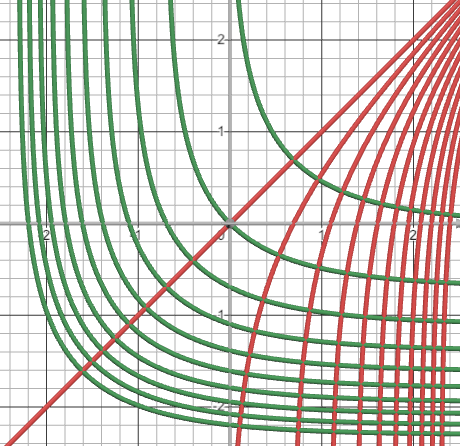
\includegraphics[width=.5\textwidth]{double.png}
\end{center}
6) Выберите какую-либо векторную линию поля и зафиксируйте на ней точки A и B, выбрав
для них числовые координаты. Вычислите работу поля вдоль этой линии, используя найденный в п. 3) потенциал.

Работа потенциального поля по кривой AB:
\begin{equation*}
    A = \int_{A}^{B}\vec{H}\cdot d\overline{l} = \mathbb{U}(B) - \mathbb{U}(A)
\end{equation*}
Фиксируем точки B(-2;0), A(0;-2), тогда:
\begin{equation*}
    A = e^{-2}-e^{0}-e^{0}+e^{-2} = -1,73 \text{ Дж}
\end{equation*}
\section*{Задание 4. Поток векторного поля}
Дано: Дано тело Т, ограниченное следующими поверхностями:
\begin{equation*}
    y+\sqrt{x^2+z^2}=0
\end{equation*}
\begin{equation*}
    x^2+y^2=1
\end{equation*}
\begin{equation*}
    x^2+y+z^2=2
\end{equation*}
На рисунке представлено сечение тела Т координатной плоскостью Oyz.
\begin{center}
    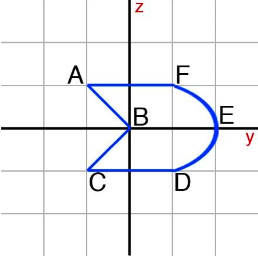
\includegraphics[width=.3\textwidth]{figure.png}
\end{center}
Решение:
\\ \\
1) Изобразите тело Т на графике в пространстве.
\begin{center}
    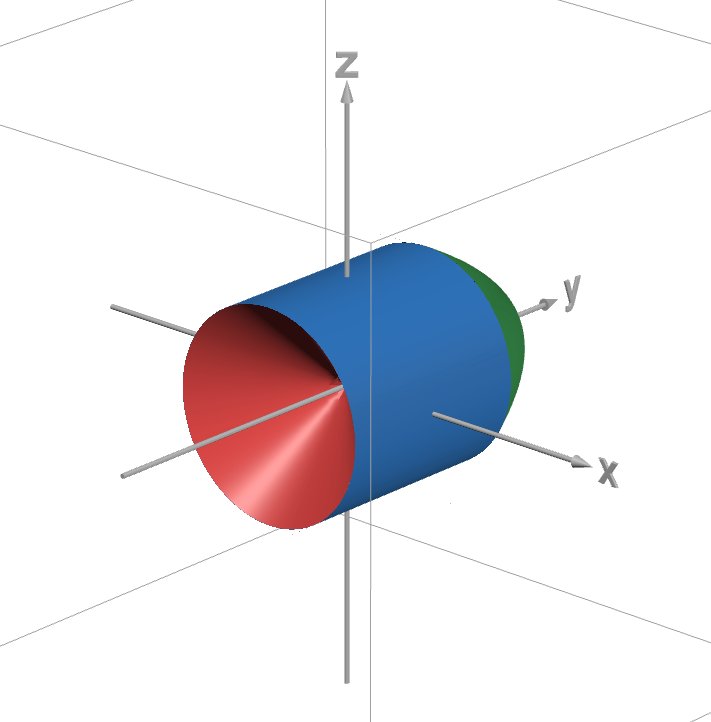
\includegraphics[width=.5\textwidth]{top.png}
\end{center}
\begin{center}
    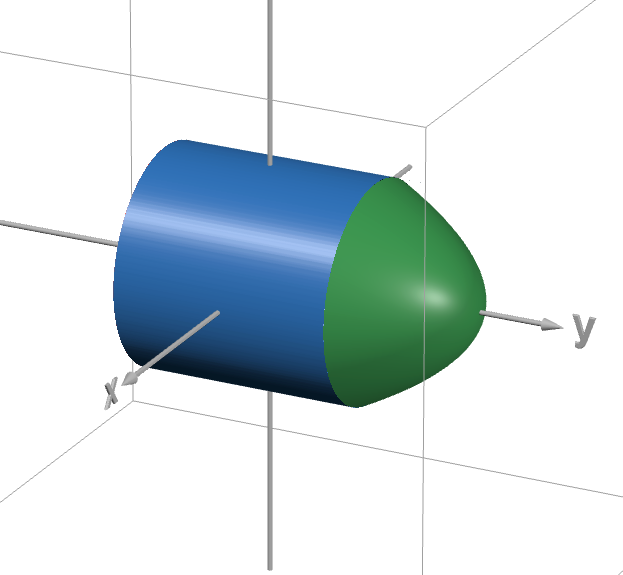
\includegraphics[width=.5\textwidth]{button.png}
\end{center}
2) Вычислите поток поля $a=(sin\ zy^2)\vec{i}+ \sqrt{2}x\vec{j}+(\sqrt{2+y}-3z)\vec{k}$ через боковую
поверхность тела T, образованную вращением дуги AFEDC вокруг оси Oy, в направлении внешней нормали поверхности тела Т.

\begin{equation*}
    \iint_{S^+}\vec{a}\cdot d\vec{S}=\iiint_Tdiv\vec{a}\cdot dV =
    \iiint_T(\pdv{sin\ zy^2}{x}+\pdv{\sqrt{2}x}{y}+\pdv{\sqrt{2+y}-3z}{z})dxdydz =
\end{equation*}
Перейдём в цилиндрическую систему координат:
\begin{equation*}
    y=y;\ x=\rho cos\phi;\ z=\rho sin\phi; |\mathbb{J}|=\rho
\end{equation*}
\begin{equation*}
    \rho^2cos^2\phi+y+\rho^2sin^2\phi =2;\ y+\rho^2=2;\ \rho^2=2-y;\ \rho = \sqrt{2-y}
\end{equation*}
\begin{equation*}
    \text{Первая фигура: }
    \begin{cases}
        -1\leq y\leq 1\\
        0\leq\rho \leq 1\\
        0\leq \phi < 2\pi
    \end{cases}
    \text{Вторая фигура: }
    \begin{cases}
        1< y\leq 2\\
        0\leq\rho \leq \sqrt{2-y}\\
        0\leq \phi < 2\pi
    \end{cases}
\end{equation*}
\begin{equation*}
    =-3\iiint_Tdxdydz = -3(\int_{-1}^{1}dy\int_{0}^{2\pi}d\phi\int_{0}^{1}\rho d\rho+\int_{1}^{2}dy\int_{0}^{2\pi}d\phi\int_{0}^{\sqrt{2-y}}\rho d\rho)=-3\pi(1-(-1)+(2\cdot 2-\frac{1}{2}\cdot 2^2-(2\cdot 1-\frac{1}{2}\cdot 1)))=
\end{equation*}
\begin{equation*}
    =-\frac{15}{2}\pi
\end{equation*}

\newpage
\section*{Задание 5. Формулы теории поля}
\textbf{
    Задание:
}

При помощи формулы Остроградского-Гаусса доказать формулу трёхмерного
интегрирования по частям:

\[\iiint_{T}^{\ }{U\mathrm{\Delta}V{dv}} = \oiint_{S}^{\ }{U\frac{\partial V}{\partial\overrightarrow{n}}dS} - \iiint_{T}^{\ }{(grad\ U \cdot grad\ V){dv}},\]

где \(T\) -- ограниченная область в пространстве с границей \(S\),

\(S\) -- гладкая односвязная поверхность,

\(U(x;\ y;\ z)\) и \(V(x;\ y;\ z)\) -- непрерывно дифференцируемые в
области \(T\) функции,

\(\frac{\partial V}{\partial\overrightarrow{n}}\ \)-- производная по
направлению нормали \(\overrightarrow{n}\) к поверхности \(S\),

\(\mathrm{\Delta}\) -- оператор Лапласа,

\(dv\  = \ dxdydz\) -- элементарный объём в области \(T\).
\\ \\
\textbf{
    Решение:
}\\ \\
1) Воспользуемся формулой Остроградского-Гаусса:

\[\oiint_{S}^{\ }{\overrightarrow{F} \cdot \overrightarrow{dS}} = \iiint_{T}^{\ }{div\ \overrightarrow{F}\ dv}\]

Применим формулу Остроградского-Гаусса к векторному полю
\(\overrightarrow{F}\  = \ U \cdot grad\ V\)

По свойству дивергенции для скалярного поля \(\varphi\) и векторного
\(F\):

\[div(\varphi F) = \frac{\partial\varphi F_{x}}{\partial x} + \frac{\partial\varphi F_{y}}{\partial y} + \frac{\partial\varphi F_{z}}{\partial z} = F_{x}\frac{\partial\varphi}{\partial x} + \varphi\frac{\partial F_{x}}{\partial x} + F_{y}\frac{\partial\varphi}{\partial y} + \varphi\frac{\partial F_{y}}{\partial y} + F_{z}\frac{\partial\varphi}{\partial z} + \varphi\frac{\partial F_{z}}{\partial z} = grad\ \varphi \cdot F + \ \varphi\ div\ F\]

\[div(\varphi F) = grad\ \varphi \cdot F + \ \varphi\ div\ F\]

Получаем:

\[div\ \overrightarrow{F} = grad\ U \cdot grad\ V + U\ div(grad\ F) =^{def} grad\ U \cdot grad\ V + U\mathrm{\Delta}V\]

\[\oiint_{S}^{\ }{U \cdot grad\ V \cdot \overrightarrow{dS}} = \iiint_{T}^{\ }{(grad\ U \cdot grad\ V + U\mathrm{\Delta}V)\ dv}\]
\\ \\
2) Разобьем тройной интеграл в правой части на тройные интегралы от
\(U\mathrm{\Delta}V\) и \(grad\ U \cdot grad\ V\). И распишем
\(\overrightarrow{dS}\) с помощью вектора нормаля и элемента площади
поверхности:

\[\iiint_{T}^{\ }{U\mathrm{\Delta}V\ dv} = \oiint_{S}^{\ }{U \cdot grad\ V \cdot \overrightarrow{n}dS} - \iiint_{T}^{\ }{(grad\ U \cdot grad\ V)\ dv}\]
\\ \\
3) При проекции вектора на плоскость мы делим скалярное произведение на
длину вектора, куда проектируем, и учитывая, что в данном случае
проектируем на единичный вектор (нормаль к плоскости), мы выражаем
\(grad\ V \cdot \overrightarrow{n}\) как производную функции по
направлению нормали к плоскости \(S\). Таким образом, получаем исходное
равенство.:

\[\iiint_{T}^{\ }{U\mathrm{\Delta}V\ dv} = \oiint_{S}^{\ }{U\frac{\partial V}{\partial\overrightarrow{n}}dS} - \iiint_{T}^{\ }{(grad\ U \cdot grad\ V)\ dv}\]

Что и требовалось доказать.



\end{document}


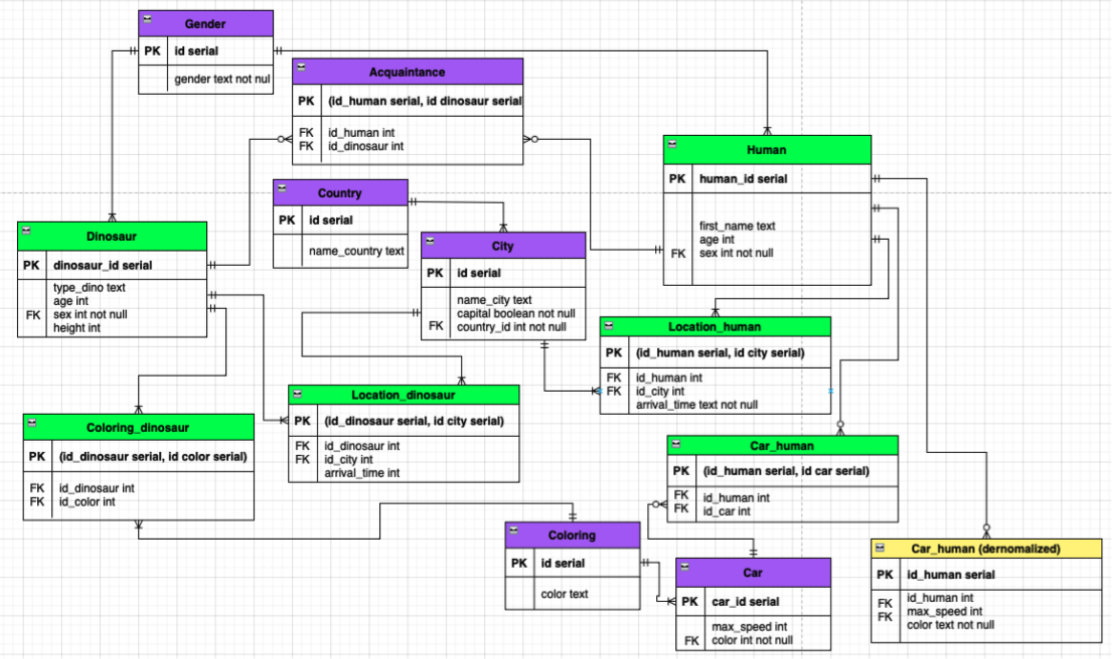
\includegraphics[width=.9\textwidth]{123}